\begin{figure}
    \centering
    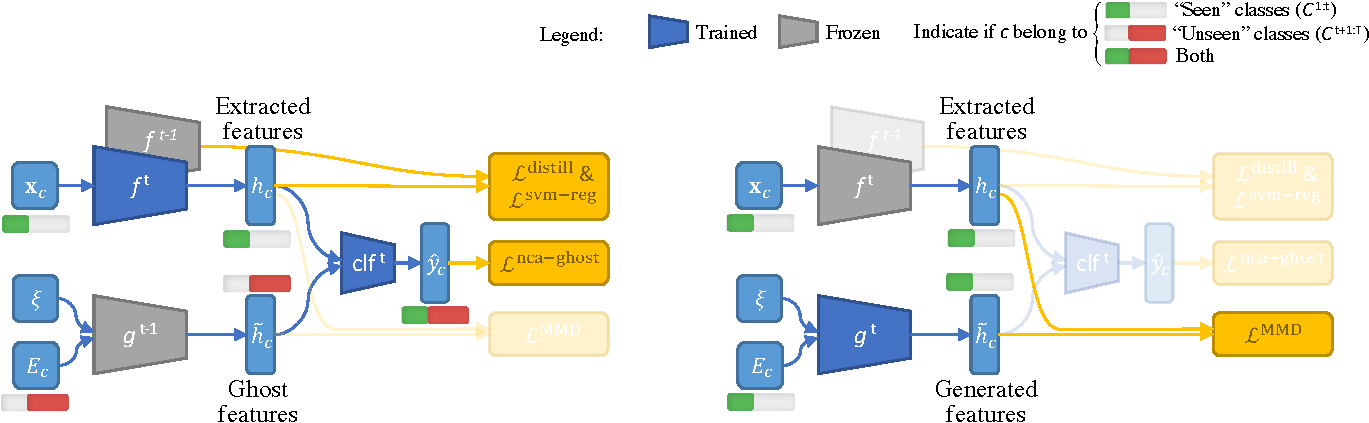
\includegraphics[width=\linewidth]{images/ghost/model.pdf}
    \begin{subfigure}{.5\textwidth}
        \vspace{2mm}
        \centering
        \caption{Training of the classifier}
        \label{fig:ghost_training_cls}
    \end{subfigure}%
    \begin{subfigure}{.5\textwidth}
        \vspace{2mm}
        \centering
        \caption{Training of the generator}
        \label{fig:ghost_training_gen}
    \end{subfigure}
    \caption{\textbf{Procedure to train our model applied at each task/step}: (a) a complete classifier is learned with seen and unseen features ($\mcL^\text{\tiny{nca-ghost}}$). The feature extractor is protected from catastrophic forgetting ($\mcL^\text{\tiny{distill}}$), and constrained to separate seen classes from unseen/ghosts classes ($\mcL^\text{\tiny{svm-reg}}$). (b) Once a task is done, the generator is fine-tuned on the new latent space ($\mcL^\text{\tiny{MMD}}$) on seen classes. Notice that for the first and last tasks, the classifier does not use the ghost features.}
    \label{fig:ghost_training_procedure}
\end{figure}
